
% TODO(Marcos): Decir por que se decidio definir un lenguaje propio y no
% utilizar los que se estudiaron anteriormente.
% Tambien decir que comparte con esos lenguajes y en que difiere.

  En este capítulo se describe el diseño del lenguaje \frob{} junto con su semántica.
  Luego se explica de qué manera es traducido al lenguaje \alf{} de
bajo nivel, mas simple de interpretar, el cual podrá ser interpretado
por implementaciones de una misma máquina virtual en diferentes
plataformas de hardware.

  También se describirán las etapas de compilación, desde que se escribe
un programa en alto nivel hasta que es ejecutado en una
plataforma objetivo.

  El diagrama de la Figura \ref{fig:compilacion} resume todas las etapas y
componentes necesarios.

\begin{figure}[h]
\begin{center}
\caption{Etapas y componentes}
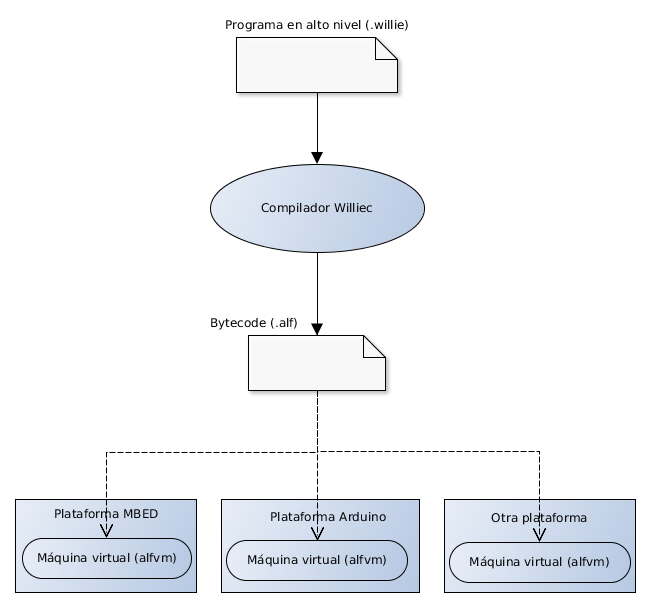
\includegraphics[width=0.9\textwidth]{graphs/compilacion.png}
\label{fig:compilacion}
\end{center}
\end{figure}

  En la parte de arriba de la Figura se ve un programa en el
lenguaje \frob{} de alto nivel.
  El desarrollador escribe dicho programa y
ejecuta el compilador \compilador{} y obtiene un archivo \alf{} binario.

  Debajo se muestran diversas plataformas, cada una
con su implementación de la máquina virtual \maquinavirtual{} instalada.

  El desarrollador podrá cargar el mismo código \alf{} en cualquier robot que
esté construido utilizando cualquiera de las plataformas, y la máquina
virtual se encargará de interpretarlo.
